% !TEX root = main.tex

There are only a few public sources for email data to which almost everyone trying to do similar analysis will turn to. For our project, we downloaded datasets from the following three locations:

\begin{enumerate}
\item Enron-Spam datasets
\item SpamAssassin data
\item TREC email corpus
\end{enumerate} 

We combine all emails and extracted the information including date, from, to, subject, content, number of cc, and number of bcc. In the process of data preprocessing, we faced some challenges to get the information of year, weekday, and hour at which the email was sent. We tried to use the string methods in python but end up finding regular expression is more powerful to extract the weekday and month. The other challenge of cleaning up the emails come from trying to remove the html and css elements, such that when we tokenize we wouldn't end up with tag elements as the most frequent words. Although we cannot remove all html and css, we did manage to get rid of most of it by the removal of contents between brackets, parathesis, and curly braces as well as words that begin with a period. \\

\begin{figure}[h]
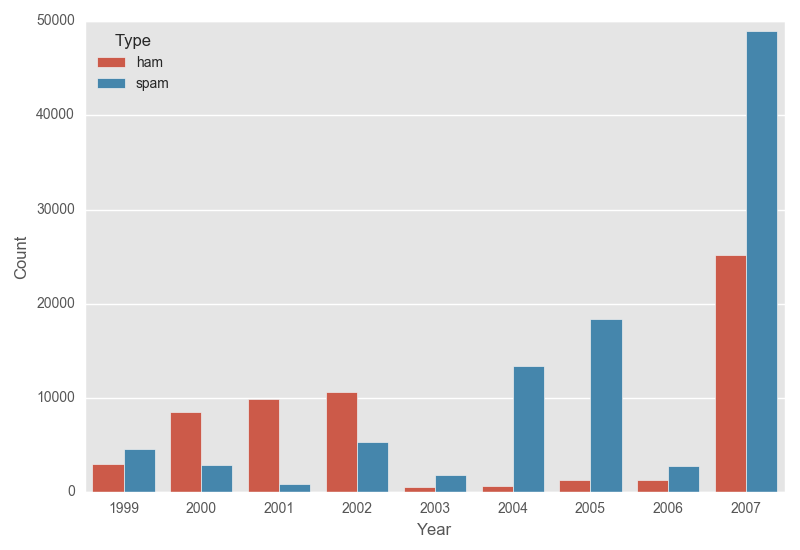
\includegraphics[width=10cm]{Email_count_each_year.png}
\centering
\caption{Amount of Email From 1999 to 2007}
\label{email_every_year}
\end{figure}

\begin{table}[h]
\centering
\caption{Proportion of Ham Email and Spam Email From 1999 to 2007}
\label{proportion_ham_spam}
\begin{tabular}{@{}llllll@{}}
\toprule
Year & Ham   & Spam  & Ham \%   & Spam \%  & Total \\ \midrule
1999 & 2978  & 4611  & 0.392410 & 0.607590 & 7589  \\
2000 & 8512  & 2851  & 0.749098 & 0.250902 & 11363 \\
2001 & 9872  & 848   & 0.920896 & 0.079104 & 10720 \\
2002 & 10663 & 5280  & 0.668820 & 0.331180 & 15943 \\
2003 & 545   & 1773  & 0.235116 & 0.764884 & 2318  \\
2004 & 627   & 13420 & 0.044636 & 0.955364 & 14047 \\
2005 & 1309  & 18418 & 0.066356 & 0.933644 & 19727 \\
2006 & 1226  & 2730  & 0.309909 & 0.690091 & 3956  \\
2007 & 25219 & 48999 & 0.339796 & 0.660204 & 74218 \\ \bottomrule
\end{tabular}
\end{table}

After finishing the data cleaning up, we delete the emails with year not between 1999 to 2007 to prevent the situation that the date of the emails is after when the data was collected and that the date of email is so early that the email are still not common used. There are 159981 email with 60951 of them are ham and the other 98930 are spam. From Table \ref{proportion_ham_spam} and Figure \ref{email_every_year}, we can see that there is a disproportional number of emails between each year as well as between spam and ham groups. The imbalance dataset may be worrisome for our classifiers. However, there is not much we can do about this situation. Maybe if we can see that there is not too much variation between ham and spam emails across years or there is no time obvious time effect on the emails, then combining the different years wouldn't be a problem. To see whether there are differences in email across the email, we will examine the top words by year. Figure \ref{email_hour_weekday} shown the amount of the email sent each hour and each day. There is a peak for sending spam email at around 12:00 to 15:00. However, ham emails were usually sent between 8:00 to 20:00. Also, according to the right plot of Figure \ref{email_hour_weekday}, ham emails tend to be sent during weekdays and has lower proportion in weekend but spam email seems to be balance each day.\\


\begin{figure}[H]
\begin{subfigure}{\textwidth}
  \centering
  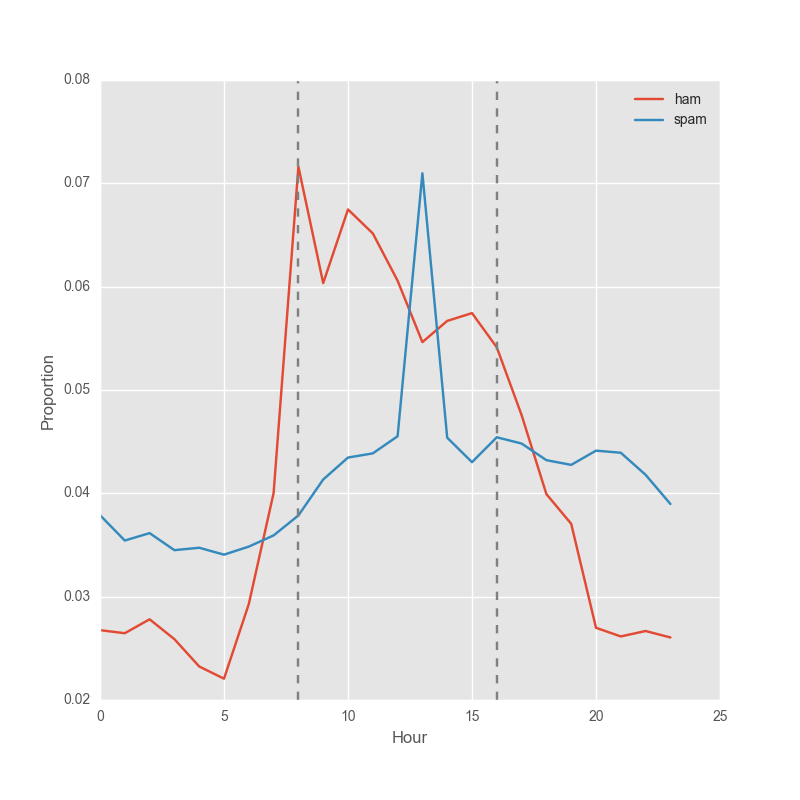
\includegraphics[width=.4\linewidth]{Ham_and_Spam_per_hour.png}
  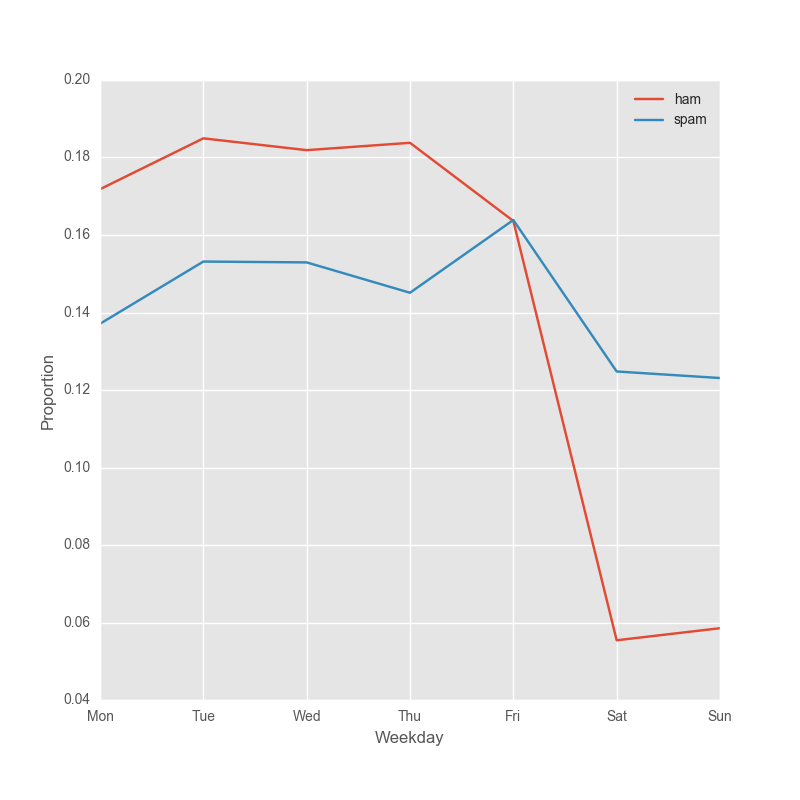
\includegraphics[width=.4\linewidth]{Ham_and_Spam_weekday.png}
\end{subfigure}%
\caption{Amount of Email Hourly and On Different Weekday}
\label{email_hour_weekday}
\end{figure}